% Options for packages loaded elsewhere
\PassOptionsToPackage{unicode}{hyperref}
\PassOptionsToPackage{hyphens}{url}
\PassOptionsToPackage{dvipsnames,svgnames,x11names}{xcolor}
%

\documentclass[
  a4paper, 
  twoside,
  final
]{article}

\usepackage{amsmath,amssymb}
\usepackage{iftex}
\ifPDFTeX
  \usepackage[T1]{fontenc}
  \usepackage[utf8]{inputenc}
  \usepackage{textcomp} % provide euro and other symbols
\else % if luatex or xetex
  \usepackage{unicode-math}
  \defaultfontfeatures{Scale=MatchLowercase}
  \defaultfontfeatures[\rmfamily]{Ligatures=TeX,Scale=1}
\fi
\usepackage{lmodern}
\ifPDFTeX\else  
    % xetex/luatex font selection
\fi
% Use upquote if available, for straight quotes in verbatim environments
\IfFileExists{upquote.sty}{\usepackage{upquote}}{}
\IfFileExists{microtype.sty}{% use microtype if available
  \usepackage[]{microtype}
  \UseMicrotypeSet[protrusion]{basicmath} % disable protrusion for tt fonts
}{}
\makeatletter
\@ifundefined{KOMAClassName}{% if non-KOMA class
  \IfFileExists{parskip.sty}{%
    \usepackage{parskip}
  }{% else
    \setlength{\parindent}{0pt}
    \setlength{\parskip}{6pt plus 2pt minus 1pt}}
}{% if KOMA class
  \KOMAoptions{parskip=half}}
\makeatother
\usepackage{xcolor}
\setlength{\emergencystretch}{3em} % prevent overfull lines
\setcounter{secnumdepth}{5}
% Make \paragraph and \subparagraph free-standing
\ifx\paragraph\undefined\else
  \let\oldparagraph\paragraph
  \renewcommand{\paragraph}[1]{\oldparagraph{#1}\mbox{}}
\fi
\ifx\subparagraph\undefined\else
  \let\oldsubparagraph\subparagraph
  \renewcommand{\subparagraph}[1]{\oldsubparagraph{#1}\mbox{}}
\fi

\usepackage{color}
\usepackage{fancyvrb}
\newcommand{\VerbBar}{|}
\newcommand{\VERB}{\Verb[commandchars=\\\{\}]}
\DefineVerbatimEnvironment{Highlighting}{Verbatim}{commandchars=\\\{\}}
% Add ',fontsize=\small' for more characters per line
\usepackage{framed}
\definecolor{shadecolor}{RGB}{241,243,245}
\newenvironment{Shaded}{\begin{snugshade}}{\end{snugshade}}
\newcommand{\AlertTok}[1]{\textcolor[rgb]{0.68,0.00,0.00}{#1}}
\newcommand{\AnnotationTok}[1]{\textcolor[rgb]{0.37,0.37,0.37}{#1}}
\newcommand{\AttributeTok}[1]{\textcolor[rgb]{0.40,0.45,0.13}{#1}}
\newcommand{\BaseNTok}[1]{\textcolor[rgb]{0.68,0.00,0.00}{#1}}
\newcommand{\BuiltInTok}[1]{\textcolor[rgb]{0.00,0.23,0.31}{#1}}
\newcommand{\CharTok}[1]{\textcolor[rgb]{0.13,0.47,0.30}{#1}}
\newcommand{\CommentTok}[1]{\textcolor[rgb]{0.37,0.37,0.37}{#1}}
\newcommand{\CommentVarTok}[1]{\textcolor[rgb]{0.37,0.37,0.37}{\textit{#1}}}
\newcommand{\ConstantTok}[1]{\textcolor[rgb]{0.56,0.35,0.01}{#1}}
\newcommand{\ControlFlowTok}[1]{\textcolor[rgb]{0.00,0.23,0.31}{#1}}
\newcommand{\DataTypeTok}[1]{\textcolor[rgb]{0.68,0.00,0.00}{#1}}
\newcommand{\DecValTok}[1]{\textcolor[rgb]{0.68,0.00,0.00}{#1}}
\newcommand{\DocumentationTok}[1]{\textcolor[rgb]{0.37,0.37,0.37}{\textit{#1}}}
\newcommand{\ErrorTok}[1]{\textcolor[rgb]{0.68,0.00,0.00}{#1}}
\newcommand{\ExtensionTok}[1]{\textcolor[rgb]{0.00,0.23,0.31}{#1}}
\newcommand{\FloatTok}[1]{\textcolor[rgb]{0.68,0.00,0.00}{#1}}
\newcommand{\FunctionTok}[1]{\textcolor[rgb]{0.28,0.35,0.67}{#1}}
\newcommand{\ImportTok}[1]{\textcolor[rgb]{0.00,0.46,0.62}{#1}}
\newcommand{\InformationTok}[1]{\textcolor[rgb]{0.37,0.37,0.37}{#1}}
\newcommand{\KeywordTok}[1]{\textcolor[rgb]{0.00,0.23,0.31}{#1}}
\newcommand{\NormalTok}[1]{\textcolor[rgb]{0.00,0.23,0.31}{#1}}
\newcommand{\OperatorTok}[1]{\textcolor[rgb]{0.37,0.37,0.37}{#1}}
\newcommand{\OtherTok}[1]{\textcolor[rgb]{0.00,0.23,0.31}{#1}}
\newcommand{\PreprocessorTok}[1]{\textcolor[rgb]{0.68,0.00,0.00}{#1}}
\newcommand{\RegionMarkerTok}[1]{\textcolor[rgb]{0.00,0.23,0.31}{#1}}
\newcommand{\SpecialCharTok}[1]{\textcolor[rgb]{0.37,0.37,0.37}{#1}}
\newcommand{\SpecialStringTok}[1]{\textcolor[rgb]{0.13,0.47,0.30}{#1}}
\newcommand{\StringTok}[1]{\textcolor[rgb]{0.13,0.47,0.30}{#1}}
\newcommand{\VariableTok}[1]{\textcolor[rgb]{0.07,0.07,0.07}{#1}}
\newcommand{\VerbatimStringTok}[1]{\textcolor[rgb]{0.13,0.47,0.30}{#1}}
\newcommand{\WarningTok}[1]{\textcolor[rgb]{0.37,0.37,0.37}{\textit{#1}}}

\providecommand{\tightlist}{%
  \setlength{\itemsep}{0pt}\setlength{\parskip}{0pt}}\usepackage{longtable,booktabs,array}
\usepackage{calc} % for calculating minipage widths
% Correct order of tables after \paragraph or \subparagraph
\usepackage{etoolbox}
\makeatletter
\patchcmd\longtable{\par}{\if@noskipsec\mbox{}\fi\par}{}{}
\makeatother
% Allow footnotes in longtable head/foot
\IfFileExists{footnotehyper.sty}{\usepackage{footnotehyper}}{\usepackage{footnote}}
\makesavenoteenv{longtable}
\usepackage{graphicx}
\makeatletter
\def\maxwidth{\ifdim\Gin@nat@width>\linewidth\linewidth\else\Gin@nat@width\fi}
\def\maxheight{\ifdim\Gin@nat@height>\textheight\textheight\else\Gin@nat@height\fi}
\makeatother
% Scale images if necessary, so that they will not overflow the page
% margins by default, and it is still possible to overwrite the defaults
% using explicit options in \includegraphics[width, height, ...]{}
\setkeys{Gin}{width=\maxwidth,height=\maxheight,keepaspectratio}
% Set default figure placement to htbp
\makeatletter
\def\fps@figure{htbp}
\makeatother

\usepackage{region,hyperref,multirow}
\definecolor{mypink}{RGB}{219, 48, 122}
\makeatletter
\makeatother
\makeatletter
\makeatother
\makeatletter
\@ifpackageloaded{caption}{}{\usepackage{caption}}
\AtBeginDocument{%
\ifdefined\contentsname
  \renewcommand*\contentsname{Table of contents}
\else
  \newcommand\contentsname{Table of contents}
\fi
\ifdefined\listfigurename
  \renewcommand*\listfigurename{List of Figures}
\else
  \newcommand\listfigurename{List of Figures}
\fi
\ifdefined\listtablename
  \renewcommand*\listtablename{List of Tables}
\else
  \newcommand\listtablename{List of Tables}
\fi
\ifdefined\figurename
  \renewcommand*\figurename{Figure}
\else
  \newcommand\figurename{Figure}
\fi
\ifdefined\tablename
  \renewcommand*\tablename{Table}
\else
  \newcommand\tablename{Table}
\fi
}
\@ifpackageloaded{float}{}{\usepackage{float}}
\floatstyle{ruled}
\@ifundefined{c@chapter}{\newfloat{codelisting}{h}{lop}}{\newfloat{codelisting}{h}{lop}[chapter]}
\floatname{codelisting}{Listing}
\newcommand*\listoflistings{\listof{codelisting}{List of Listings}}
\makeatother
\makeatletter
\@ifpackageloaded{caption}{}{\usepackage{caption}}
\@ifpackageloaded{subcaption}{}{\usepackage{subcaption}}
\makeatother
\makeatletter
\@ifpackageloaded{tcolorbox}{}{\usepackage[skins,breakable]{tcolorbox}}
\makeatother
\makeatletter
\@ifundefined{shadecolor}{\definecolor{shadecolor}{rgb}{.97, .97, .97}}
\makeatother
\makeatletter
\makeatother
\makeatletter
\makeatother
\ifLuaTeX
  \usepackage{selnolig}  % disable illegal ligatures
\fi
\usepackage[]{natbib}
\bibliographystyle{region}
\IfFileExists{bookmark.sty}{\usepackage{bookmark}}{\usepackage{hyperref}}
\IfFileExists{xurl.sty}{\usepackage{xurl}}{} % add URL line breaks if available
\urlstyle{same} % disable monospaced font for URLs
\hypersetup{
  pdftitle={A practical guide to spatial interaction modelling},
  pdfauthor={Blinded},
  pdfkeywords={spatial interaction modelling, gravity modelling, flow
data},
  colorlinks=true,
  linkcolor={blue},
  filecolor={Maroon},
  citecolor={Blue},
  urlcolor={blue},
  pdfcreator={LaTeX via pandoc}}



\title{A practical guide to spatial interaction modelling}
\author{%
Blinded\parnote{}}
\date{}

\setcounter{page}{999}
\renewcommand{\thepage}{\arabic{page}}  % L for Letters, R for Resources, E for Editorial
\jvol{1} 
\jnum{1} 
\jyear{2020} 
\jpages{999--999} 
\jauthor{MISSING} 
\received{} 
\accepted{} 

\jdoi{10.18335/region.v??i??.???} 

\setlength{\parskip}{0pt plus1pt}
\setlength{\parindent}{15pt}

% %\bibliographystyle{plainnat}
\bibpunct{(}{)}{,}{a}{}{,}   % % changes formatting in natbib, see http://merkel.zoneo.net/Latex/natbib.php
% % It can be moved into the package call!

%%%%%%%%%%% GM inserted %%%%%%%%%%%%%%%
\usepackage[breakable]{tcolorbox}

% prompt
\makeatletter
\newcommand{\boxspacing}{\kern\kvtcb@left@rule\kern\kvtcb@boxsep}
\makeatother
\newcommand{\prompt}[4]{
	\ttfamily\llap{{\color{#2}[#3]:\hspace{3pt}#4}}\vspace{-\baselineskip}
}

\definecolor{incolor}{HTML}{303F9F}
\definecolor{outcolor}{HTML}{D84315}
\definecolor{cellborder}{HTML}{CFCFCF}
\definecolor{cellbackground}{HTML}{F7F7F7}
\definecolor{celloutborder}{HTML}{FFAFAF}
\definecolor{celloutbackground}{HTML}{F7E7E7}

\newcounter{code}
%%%%%%%%%%%%%%%%%%%%%%%%%%%%%%%%%%%%%%%

\newenvironment{ROutput}{\definecolor{shadecolor}{HTML}{F7E7E7}\begin{snugshade}}{\end{snugshade}}
\newenvironment*{RInput}{}{}
\begin{document}
\maketitle
\begin{abstract}
This document is only a demo explaining how to use the template.
\end{abstract}
\ifdefined\Shaded\renewenvironment{Shaded}{\begin{tcolorbox}[boxrule=0pt, enhanced, interior hidden, sharp corners, borderline west={3pt}{0pt}{shadecolor}, breakable, frame hidden]}{\end{tcolorbox}}\fi

\hypertarget{sec-intro}{%
\section{Introduction}\label{sec-intro}}

Spatial interaction models (SIMs) is a core tool to simulate flows
between different locations in physical space. They are a valuable
resource through which the geographic structure between locations
encoded in aggregate flows of people, information and goods can be
represented and understood. Intuitively, SIMs seek to capture the
spatial interaction between places as a function of three components:
origin attributes, destination attributes and their separation. Inspired
by Newtonian concepts developed in physics, spatial flows between
locations are conceived as the result of their proportional
gravitational force and inverse association with spatial separation.
Attributes of origin and destination locations are employed to represent
gravitational forces pushing and pulling people, information and goods
between specific locations. Various forms of distance and costs are used
to represent the deterring effects of geographical separation on spatial
flows.

SIMs are widely used for prediction and inference. They are used to make
inference about the factors contributing to influence spatial flows.
They have been used to understand the magnitude and direction of
influence of individual and place-level attributes on geographic flows.
Understanding the effect of these factors offers valuable evidence to
inform the development of appropriate plans, strategies and
interventions \citep{fotheringham_okelly1989}. SIMs are also used to
make predictions of the size of spatial flows. These predictions are
normally used to assess the impact of interventions and creation of
``what-if'' scenarios, providing guidance for the identification of
optimal locations and size for potential new service units {[}REF{]}. In
this context, SIMs are often used to evaluate the impact of new bus
stops, shopping stores, schools or housing units on their potential
demand and traffic changes \citep{fotheringham_okelly1989}. To these
ends, SIMs have been used to address questions in a variety of settings,
including retail, migration, transport, trade, commuting, school travel
and more broadly urban planning.

Yet, the implementation of SIMs remains a challenge. Algorithms to
calibrate the parameters of SIMs have remained locked away, either
behind dense algebraic notation in dusty papers from the 1970s, or
behind paywalls of commercial software \citep{rowe2024}. Additionally,
\citet{rowe2024} noted a dearth of knowledge within geographical
education as SIMs are not widely taught in undergraduate programmes in
the same way as, for instance, regression models are taught in economics
or social psychology. This situation is argued to have occurred despite
the availability of effective routines to calibrate SIMs via popular
linear and general linear modelling frameworks, and as practical
expediency is sacrificed at the expense of theoretical or technical
prowess \citep{rowe2024}. The ways in which calibration procedures are
presented as lengthy mathematical derivation or passing reference to
ordinary least square tend to hamper accessibility for the easy
implementation of SIMs.

This computational notebook contributes to redressing these issues. It
aims to provide an intuitive, understandable and practical guide to
estimate SIMs in a variety of modelling frameworks. It will include the
necessary code to calibrate SIMs, using origin-destination
travel-to-work data for the United Kingdom in R programming language.
The code provided is generisable and can be adapted to different
origin-destination flow data and contexts, including migration, student,
transport, trade, currency, data transfer, vessel, shipment and freight
flows.

The notebook is structured as follows. The next section sets out some
fundamental concepts and definitions relating to SIMs.
Section~\ref{sec-comenv} identifies the libraries used before
Section~\ref{sec-data} describes the data. Section~\ref{sec-visualising}
illustrates key techniques to visualise complex spatial interaction
data, and Section~\ref{sec-modelling} shows and explains how to estimate
SIMs using a range of modelling frameworks. It start with traditional
mathematical and Ordinary Least Squares (OLS) approaches to more
advanced statistical frameworks, such as Generalised Linear Mixed Models
(GLMMs) and machine learning algorithms.

\hypertarget{context}{%
\section{Context}\label{context}}

SIMs take various forms. Newtonian gravity models are probably the most
widely known and used form of SIMs. Inspired by Newton's law of gravity,
the basic gravity version of these models assumes that the spatial flows
or interactions between an origin (\(i\)) and a destination \(j\) is
proportional to their masses (\(M_{i}\) and \(M_{j}\)) and inversely
proportional to their separation (\(D_{ij}\)). Locations are expected to
interact in a positively reinforcing manner that is multiplicative of
their masses, but to diminish with the intervening role of their
separation. The parameters \(\mu\) and \(\gamma\) reflect the
proportional relationship between the masses and flows. The separation
between locations is often represented by a distance decay function and
is measured in terms of the distance, cost or time involved in the
interaction. Generally, the model includes a constant (\(\kappa\))
ensuring that the expected flows do not exceed their respective observed
counts, and a parameter (\(\beta\)) representing the deterring effect of
geographical separation. The task is to estimate the parameters
\(\kappa\), \(\mu\), \(\gamma\) and \(\beta\). Following
\citet{wilson1971}, a gravity model can be expressed as:

\begin{equation}\protect\hypertarget{eq-1}{}{
T_{ij} = \kappa \frac{M^{\mu}_{i} M^{\gamma}_{j}}{D^{\beta}_{ij} }
}\label{eq-1}\end{equation}

SIMs have three key inputs: (1) a matrix of flows between a set of
origins and destinations; (2) a measure of separation between origins
and destinations; and, (3) measures of masses at origin and destination
locations. The literature usually considers a family of SIMs taking four
forms which refers to various constraints placed on parameters of the
model \citep{wilson1971}. There is an \emph{unconstrained} version which
offers a measure of spatial separation, assuming that there is no
information on the number of flows originating from each origin to each
destination. The number of flows is thus estimated via SIMs using
surrogate factors, such as population at the origin and destiination.
Constrained versions are used to ensure that specific origin or
destination observations are met. Three general formulations of
constrained models are used: \emph{production-constrained},
\emph{attraction-constrained} and \emph{doubly-constrained} models.
\emph{Production-constrained} versions are used to constrain a model to
origin factors so that the predicted flows emanating from individual
origins are in proportion to the relative attractiveness of each
destination. \emph{Attraction-constrained} versions do the same but
constrain models to destination factors so that the predicted flows
terminating at each destination are in proportion to the relative
attactiveness at individual origins. \emph{Doubly-constrained} versions
combine these two sets of constraints to ensure predicted flows are
equal to observed flows are constrained by both origin and destination
factors.

Various modelling frameworks have been used to calibrate the parameters
of SIMs. Originally, mathematical formulations were heavily used but
these did not offer any ideas of uncertainty about the estimated
parameters and were seen as deterministic. To mitigate this, statistical
frameworks proliferated. A simple and widely used formulation is a
linear model in which geographic flows are logged to meet the normality
modelling assumptions, and OLS and maximum likelihood optimisation
frameworks are used to estimate the model parameters. However, linear
modelling has various constraints and cannot easily incorporate flow
counts of zero, right-skewed distributions of flows and non-linear
relationships between flows and the set of predictors. As result, more
advanced modelling frameworks have been used to fit SIMs, including
count data approaches such as Poison and Negative Binomial Models
\citep{rowe2023urban}, Generalised Linear Mixed Models
\citep{apariciocastro2023} and more recently machine learning
\citep{rowe2022} and deep learning models \citep{simini2021}. This
computational notebook will provide a practical guide on how to
implement these models using travel-to-work data for the UK. The next
sections will first introduce the computational environment and data
used for this purpose.

\hypertarget{sec-comenv}{%
\section{Computation environment}\label{sec-comenv}}

\begin{Shaded}
\begin{Highlighting}[]
\CommentTok{\# data management }
\FunctionTok{library}\NormalTok{(tidyverse)}
\CommentTok{\# spatial data management}
\FunctionTok{library}\NormalTok{(sf)}
\CommentTok{\# generalised mixed linear modelling}
\FunctionTok{library}\NormalTok{(glmmTMB)}
\CommentTok{\# data visualisation}
\FunctionTok{library}\NormalTok{(scales)}
\FunctionTok{library}\NormalTok{(patchwork)}
\FunctionTok{source}\NormalTok{(}\StringTok{"../../code/style/data{-}visualisation\_theme.R"}\NormalTok{)}
\end{Highlighting}
\end{Shaded}

\hypertarget{sec-data}{%
\section{Data}\label{sec-data}}

We use an origin-destination matrix capturing travel-to-work commuting
flows from the 2021 Census for England and Wales. The data provide
estimates on usual residents aged 16 years and over and in employment
before the Census week at the Lower Tier Local Authority (LTLA) level.
The estimates capture the movement of people between their LTLA area of
residence and work. The data are available in a long origin-destination
pair format. The first seven columns contain the core components of a
spatial interaction dataset, including code and names for origin and
destination locations, and the population count moving between a
origin-destination pair. The remainder of the dataset comprises the
origin and destination attributes, including the total population count
and population counts by socioeconomic categories. Columns 9 to 19
contain the attributes at origins and columns 20 to 31 contain the
attributes at destinations. Looking at the data frame vertically, the
first row shown below displays the count of people who reported
Hartlepool as their place of residence and work. The third row shows the
count of people who were residing in Hartlepool but reported to travel
to work in Middlesbrough.

\begin{Shaded}
\begin{Highlighting}[]
\CommentTok{\# read data}
\NormalTok{df }\OtherTok{\textless{}{-}} \FunctionTok{read\_csv}\NormalTok{(}\StringTok{"../../data/output/sim\_uk{-}travel{-}to{-}work\_2021.csv"}\NormalTok{) }\SpecialCharTok{\%\textgreater{}\%} 
  \CommentTok{\# rename variables}
  \FunctionTok{rename}\NormalTok{(}
    \AttributeTok{ltla\_res\_code =} \StringTok{"Lower tier local authorities code"}\NormalTok{,}
    \AttributeTok{ltla\_res\_name =} \StringTok{"Lower tier local authorities label"}\NormalTok{,}
    \AttributeTok{ltla\_work\_code =} \StringTok{"LTLA of workplace code"}\NormalTok{,}
    \AttributeTok{ltla\_work\_name =} \StringTok{"LTLA of workplace label"}\NormalTok{,}
    \AttributeTok{ltla\_work\_id\_code =} \StringTok{"Place of work indicator (4 categories) code"}\NormalTok{,}
    \AttributeTok{ltla\_work\_id\_lbl =} \StringTok{"Place of work indicator (4 categories) label"}\NormalTok{,}
    \AttributeTok{count =} \StringTok{"Count"}
\NormalTok{  ) }\SpecialCharTok{\%\textgreater{}\%} 
  \CommentTok{\# exclude the following observations:}
\NormalTok{  dplyr}\SpecialCharTok{::}\FunctionTok{filter}\NormalTok{(}\SpecialCharTok{!}\NormalTok{ltla\_work\_name }\SpecialCharTok{\%in\%} 
                  \FunctionTok{c}\NormalTok{(}\StringTok{"Does not apply"}\NormalTok{, }
                    \StringTok{"Workplace is offshore installation"}\NormalTok{, }
                    \StringTok{"Workplace is outside the UK"}\NormalTok{) ) }\SpecialCharTok{\%\textgreater{}\%} 
  \CommentTok{\# exclude the following variables:}
  \FunctionTok{select}\NormalTok{( }\SpecialCharTok{{-}}\FunctionTok{c}\NormalTok{(ltla\_work\_id\_code, ltla\_work\_id\_lbl) ) }\SpecialCharTok{\%\textgreater{}\%} 
  \CommentTok{\# exclude stayers}
\NormalTok{  dplyr}\SpecialCharTok{::}\FunctionTok{filter}\NormalTok{(ltla\_res\_code }\SpecialCharTok{!=}\NormalTok{ ltla\_work\_code) }
\FunctionTok{head}\NormalTok{(df, }\AttributeTok{n =} \DecValTok{5}\NormalTok{ ) }
\end{Highlighting}
\end{Shaded}

\begin{verbatim}
# A tibble: 5 x 31
  ltla_res_code ltla_res_name ltla_work_code ltla_work_name   count population_o
  <chr>         <chr>         <chr>          <chr>            <dbl>        <dbl>
1 E06000001     Hartlepool    E06000002      Middlesbrough     1500        92338
2 E06000001     Hartlepool    E06000003      Redcar and Clev~   671        92338
3 E06000001     Hartlepool    E06000004      Stockton-on-Tees  4240        92338
4 E06000001     Hartlepool    E06000005      Darlington         398        92338
5 E06000001     Hartlepool    E06000007      Warrington           2        92338
# i 25 more variables: higher_managerial_administrative_professional_o <dbl>,
#   lower_managerial_administrative_professional_o <dbl>, intermediate_o <dbl>,
#   small_employers_own_account_o <dbl>, lower_supervisory_technical_o <dbl>,
#   semi_routine_o <dbl>, routine_o <dbl>, never_worked_unemployed_o <dbl>,
#   ft_students_o <dbl>, no_qualifications_o <dbl>, level4_o <dbl>,
#   population_d <dbl>, higher_managerial_administrative_professional_d <dbl>,
#   lower_managerial_administrative_professional_d <dbl>, ...
\end{verbatim}

\hypertarget{sec-visualising}{%
\section{Visualising spatial interaction data}\label{sec-visualising}}

\hypertarget{sec-modelling}{%
\section{Estimating spatial interaction models}\label{sec-modelling}}

This section focuses on how to calibrate spatial interaction models in
the form of gravity models. We use population at the origin and
destination to represent the mass parameters and distance between
centroids. However, the mass parameters should be thought as wider
concepts capturing the broad set of factors that may at work operating
to push flows away from origins and pulling flows towards destinations.
Similarly, distance is a broad concept capturing the cost of spatial
separation and could be measured by geographical distance, monetary,
social and phsysological cost. The section starts with the classical
mathematical formulation, then moves to basic statistical frameworks and
their extensions.

\hypertarget{mathematical-gravity-models}{%
\subsection{Mathematical gravity
models}\label{mathematical-gravity-models}}

\hypertarget{unconstrained-model}{%
\subsubsection{Unconstrained model}\label{unconstrained-model}}

We start by implementing the mathematical formulation of gravity models
using Equation~\ref{eq-1}. We adopt the standard Newtonian formulation
assuming that \(\mu\) and \(\gamma\) equal to 1 and \(\beta\) to -2, and
fit an \emph{unconstrained} model. Recall here that this model assumes
that no information on flows is available. We use the population at
origin and destination LDAs and distance between LDA centroids in
kilometers to define this model. To assess the model's predictive
capacity, we graphically compare predicted flows \emph{versus} observed
flows. We focus on movements between LDAs, removing movements within
LDAs with distance zero. A perfect model would product predicted flows
displaying a perfect positive linear relationship with the orbserved
flows. The figure below shows the unconstrained model results displaying
little correspondence between the predicted and observed flows. The
model predicts unrealistic flows of over 10 million which exceeds the
size of the observed flows. This reflects the unconstrained nature of
the model producing predictions based on distance, origin and
destination only.

\begin{figure}

{\centering 

\begin{Shaded}
\begin{Highlighting}[]
\CommentTok{\# Unconstrained model}
\CommentTok{\# assuming these parameters}
\NormalTok{mu }\OtherTok{\textless{}{-}} \DecValTok{1}
\NormalTok{gamma }\OtherTok{\textless{}{-}} \DecValTok{1}
\NormalTok{beta }\OtherTok{\textless{}{-}} \DecValTok{2}
\NormalTok{kappa }\OtherTok{\textless{}{-}} \DecValTok{1}

\CommentTok{\# using equation 1 to estimate unconstrained model}
\NormalTok{df}\SpecialCharTok{$}\NormalTok{predicted\_flow }\OtherTok{\textless{}{-}} \FunctionTok{round}\NormalTok{( kappa }\SpecialCharTok{*}
\NormalTok{  (df}\SpecialCharTok{$}\NormalTok{population\_o}\SpecialCharTok{\^{}}\NormalTok{mu }\SpecialCharTok{*}\NormalTok{ df}\SpecialCharTok{$}\NormalTok{population\_d}\SpecialCharTok{\^{}}\NormalTok{gamma) }\SpecialCharTok{/}\NormalTok{ (df}\SpecialCharTok{$}\NormalTok{distance\_km}\SpecialCharTok{\^{}}\NormalTok{beta) }
\NormalTok{  )}

\CommentTok{\# predicted versus observed flows}
\NormalTok{df }\SpecialCharTok{\%\textgreater{}\%} 
  \CommentTok{\# remove predictions}
  \FunctionTok{filter}\NormalTok{( distance\_km }\SpecialCharTok{!=} \DecValTok{0}\NormalTok{) }\SpecialCharTok{\%\textgreater{}\%} 
  \FunctionTok{ggplot}\NormalTok{( }\FunctionTok{aes}\NormalTok{( }\AttributeTok{x =}\NormalTok{ count, }\AttributeTok{y =}\NormalTok{ predicted\_flow)) }\SpecialCharTok{+}
  \FunctionTok{geom\_point}\NormalTok{( }\AttributeTok{alpha =}\NormalTok{ .}\DecValTok{5}\NormalTok{, }\AttributeTok{colour =} \StringTok{"darkblue"}\NormalTok{,}
              \FunctionTok{aes}\NormalTok{( }\AttributeTok{size =} \FunctionTok{abs}\NormalTok{(population\_o }\SpecialCharTok{/} \FloatTok{1e1}\NormalTok{)) ) }\SpecialCharTok{+}
  \CommentTok{\# change axis label to a shorthand}
  \FunctionTok{scale\_y\_continuous}\NormalTok{(}
    \AttributeTok{labels =} \FunctionTok{label\_number}\NormalTok{(}\AttributeTok{scale\_cut =} \FunctionTok{cut\_short\_scale}\NormalTok{())}
\NormalTok{    ) }\SpecialCharTok{+} 
  \FunctionTok{scale\_x\_continuous}\NormalTok{(}
    \AttributeTok{labels =} \FunctionTok{label\_number}\NormalTok{(}\AttributeTok{scale\_cut =} \FunctionTok{cut\_short\_scale}\NormalTok{())}
\NormalTok{    ) }\SpecialCharTok{+} 
  \CommentTok{\# change colour scale}
  \CommentTok{\# scale\_colour\_distiller(palette = "RdBu", direction = {-}1) +}
  \FunctionTok{labs}\NormalTok{(}\AttributeTok{y =} \StringTok{"Predicted flow"}\NormalTok{,}
       \AttributeTok{x =} \StringTok{"Observed flow"}\NormalTok{) }\SpecialCharTok{+}
  \FunctionTok{theme\_plot\_tufte}\NormalTok{() }\SpecialCharTok{+}
  \FunctionTok{theme}\NormalTok{(}\AttributeTok{legend.position =} \StringTok{"none"}\NormalTok{,}
        \AttributeTok{axis.text.y =} \FunctionTok{element\_text}\NormalTok{(}\AttributeTok{size =} \DecValTok{9}\NormalTok{),}
        \AttributeTok{axis.text.x =} \FunctionTok{element\_text}\NormalTok{(}\AttributeTok{size =} \DecValTok{9}\NormalTok{),}
        \AttributeTok{axis.title=}\FunctionTok{element\_text}\NormalTok{(}\AttributeTok{size =} \DecValTok{11}\NormalTok{)}
\NormalTok{        )}
\end{Highlighting}
\end{Shaded}

\begin{figure}[H]

{\centering 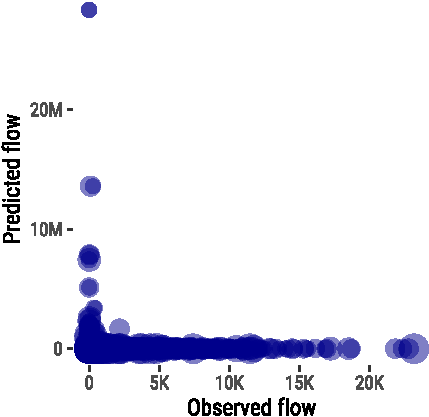
\includegraphics{region-quarto-template_files/figure-pdf/unnamed-chunk-4-1.pdf}

}

\end{figure}

Note: Colour represents the size of observed counts. Point size
represents the size of population at origins.

}

\caption{\label{fig-1}Unconstrained model predicted versus observed
flows}

\end{figure}

\hypertarget{constrained-models}{%
\subsubsection{Constrained models}\label{constrained-models}}

\emph{Production-constrained model}

To address these inconsistencies, we turn to constrained models and
first focus on the production-constrained model. This model assumes that
we observe the total flows from each origin but not those arriving in
each destination. So we can use information on the total number of
outflows to constrain the model and distribute the total outflows
proportionally to the population of destinations, and as before,
inversely proportional to distance.

\begin{Shaded}
\begin{Highlighting}[]
\CommentTok{\# Production{-}constrained model}
\CommentTok{\# total outflow from each origin}
\NormalTok{outflow }\OtherTok{\textless{}{-}}\NormalTok{ df }\SpecialCharTok{\%\textgreater{}\%}
  \FunctionTok{group\_by}\NormalTok{(ltla\_res\_code) }\SpecialCharTok{\%\textgreater{}\%}
  \FunctionTok{summarize}\NormalTok{(}\AttributeTok{total\_outflow =} \FunctionTok{sum}\NormalTok{(count)) }\SpecialCharTok{\%\textgreater{}\%} 
  \FunctionTok{ungroup}\NormalTok{()}

\CommentTok{\# merge outflows with original data}
\NormalTok{df }\OtherTok{\textless{}{-}}\NormalTok{ df }\SpecialCharTok{\%\textgreater{}\%}
  \FunctionTok{left\_join}\NormalTok{(outflow, }\AttributeTok{by =} \StringTok{"ltla\_res\_code"}\NormalTok{)}

\CommentTok{\# compute denominator for each origin}
\NormalTok{df }\OtherTok{\textless{}{-}}\NormalTok{ df }\SpecialCharTok{\%\textgreater{}\%}
  \FunctionTok{group\_by}\NormalTok{(ltla\_res\_code) }\SpecialCharTok{\%\textgreater{}\%}
  \FunctionTok{mutate}\NormalTok{(}
    \AttributeTok{kappa\_production =} 
      \FunctionTok{sum}\NormalTok{((population\_d}\SpecialCharTok{\^{}}\NormalTok{gamma) }\SpecialCharTok{/}\NormalTok{ (distance\_km}\SpecialCharTok{\^{}}\NormalTok{beta), }
                           \AttributeTok{na.rm =} \ConstantTok{TRUE}\NormalTok{)) }\SpecialCharTok{\%\textgreater{}\%}
  \FunctionTok{ungroup}\NormalTok{()}

\CommentTok{\# compute predicted flows}
\NormalTok{df }\OtherTok{\textless{}{-}}\NormalTok{ df }\SpecialCharTok{\%\textgreater{}\%} \FunctionTok{mutate}\NormalTok{(}
  \AttributeTok{production\_constrained\_flow =} 
\NormalTok{    total\_outflow }\SpecialCharTok{*}\NormalTok{ ((population\_d}\SpecialCharTok{\^{}}\NormalTok{gamma) }\SpecialCharTok{/}\NormalTok{ (distance\_km}\SpecialCharTok{\^{}}\NormalTok{beta)) }\SpecialCharTok{/} 
\NormalTok{    kappa\_production}
\NormalTok{  )}
\end{Highlighting}
\end{Shaded}

\emph{Attraction-constrained model}

Alternatively, we could assume we only have data on the total number of
flows arriving at each destination but we have no information on the
number of flows being generated from each origin. In such situations, we
can use an attraction-constrained model as it uses the known information
on total inflows for individual destinations and a set of surrogate
variables to represent the total number of flows from each origin.

\begin{Shaded}
\begin{Highlighting}[]
\CommentTok{\# Attraction{-}constrained model}
\CommentTok{\# total inflow from each origin}
\NormalTok{inflow }\OtherTok{\textless{}{-}}\NormalTok{ df }\SpecialCharTok{\%\textgreater{}\%}
  \FunctionTok{group\_by}\NormalTok{(ltla\_work\_code ) }\SpecialCharTok{\%\textgreater{}\%}
  \FunctionTok{summarize}\NormalTok{(}\AttributeTok{total\_inflow =} \FunctionTok{sum}\NormalTok{(count)) }\SpecialCharTok{\%\textgreater{}\%} 
  \FunctionTok{ungroup}\NormalTok{()}

\CommentTok{\# merge inflows with original data}
\NormalTok{df }\OtherTok{\textless{}{-}}\NormalTok{ df }\SpecialCharTok{\%\textgreater{}\%}
  \FunctionTok{left\_join}\NormalTok{(inflow, }\AttributeTok{by =} \StringTok{"ltla\_work\_code"}\NormalTok{)}

\CommentTok{\# compute denominator for each destination}
\NormalTok{df }\OtherTok{\textless{}{-}}\NormalTok{ df }\SpecialCharTok{\%\textgreater{}\%}
  \FunctionTok{group\_by}\NormalTok{(ltla\_work\_code) }\SpecialCharTok{\%\textgreater{}\%}
  \FunctionTok{mutate}\NormalTok{(}
    \AttributeTok{kappa\_attraction =} 
      \FunctionTok{sum}\NormalTok{((population\_o}\SpecialCharTok{\^{}}\NormalTok{mu) }\SpecialCharTok{/}\NormalTok{ (distance\_km}\SpecialCharTok{\^{}}\NormalTok{beta))) }\SpecialCharTok{\%\textgreater{}\%}
  \FunctionTok{ungroup}\NormalTok{()}

\CommentTok{\# compute predicted flows}
\NormalTok{df }\OtherTok{\textless{}{-}}\NormalTok{ df }\SpecialCharTok{\%\textgreater{}\%} \FunctionTok{mutate}\NormalTok{(}
  \AttributeTok{attraction\_constrained\_flow =}
\NormalTok{    total\_inflow }\SpecialCharTok{*}\NormalTok{ ((population\_o}\SpecialCharTok{\^{}}\NormalTok{mu) }\SpecialCharTok{/}\NormalTok{ (distance\_km}\SpecialCharTok{\^{}}\NormalTok{beta)) }\SpecialCharTok{/} 
\NormalTok{    kappa\_attraction}
\NormalTok{  )}
\end{Highlighting}
\end{Shaded}

\emph{Doubly-constrained model}

We can also adjust the number of flows so that both total outflows from
each origin and total inflows to each destination match observed totals.
This model requires an iterative solution to meet these constraints. To
this end, we first set the parameters for the algorithm to converge to a
solution i.e.~tolerance, maximum iterations (max\_iter) and iteration
steps (iter). Intuitively the algorithm iteratively adjust the flows by
first applying the production constrain, and subsequently the attraction
constrain in a similar manner as used above. It then assesses the
difference between total predicted and observed flows. It stops when
this difference is smaller than the established tolerance parameter. The
algorithm uses the unconstrained model predicted flow as a starting
point for the iterative process.

\begin{Shaded}
\begin{Highlighting}[]
\CommentTok{\# Doubly{-}constrained model}
\CommentTok{\# set parameters for iterations}
\NormalTok{tolerance }\OtherTok{\textless{}{-}} \FloatTok{1e{-}6}
\NormalTok{max\_iter }\OtherTok{\textless{}{-}} \DecValTok{1000}
\NormalTok{iter }\OtherTok{\textless{}{-}} \DecValTok{1}
\NormalTok{converged }\OtherTok{\textless{}{-}} \ConstantTok{FALSE}

\CommentTok{\# iteratively adjust flows to satisfy both constraints}
\ControlFlowTok{while}\NormalTok{ (}\SpecialCharTok{!}\NormalTok{converged }\SpecialCharTok{\&\&}\NormalTok{ iter }\SpecialCharTok{\textless{}=}\NormalTok{ max\_iter) \{}
  \CommentTok{\# Step 1: apply production constraint for each origin}
\NormalTok{  df }\OtherTok{\textless{}{-}}\NormalTok{ df }\SpecialCharTok{\%\textgreater{}\%}
    \FunctionTok{group\_by}\NormalTok{(ltla\_res\_code ) }\SpecialCharTok{\%\textgreater{}\%}
    \FunctionTok{mutate}\NormalTok{(}
      \AttributeTok{predicted\_flow =} 
\NormalTok{        predicted\_flow }\SpecialCharTok{*}\NormalTok{ (total\_outflow }\SpecialCharTok{/} \FunctionTok{sum}\NormalTok{(predicted\_flow))) }\SpecialCharTok{\%\textgreater{}\%}
    \FunctionTok{ungroup}\NormalTok{()}
  
  \CommentTok{\# Step 2: apply attraction constraint for each destination}
\NormalTok{  df }\OtherTok{\textless{}{-}}\NormalTok{ df }\SpecialCharTok{\%\textgreater{}\%}
    \FunctionTok{group\_by}\NormalTok{(ltla\_work\_code) }\SpecialCharTok{\%\textgreater{}\%}
    \FunctionTok{mutate}\NormalTok{(}
      \AttributeTok{predicted\_flow =} 
\NormalTok{        predicted\_flow }\SpecialCharTok{*}\NormalTok{ (total\_inflow }\SpecialCharTok{/} \FunctionTok{sum}\NormalTok{(predicted\_flow))) }\SpecialCharTok{\%\textgreater{}\%}
    \FunctionTok{ungroup}\NormalTok{()}

  \CommentTok{\# assess convergence comparing row sums of predicted and observed flows}
\NormalTok{  origin\_check }\OtherTok{\textless{}{-}}\NormalTok{ df }\SpecialCharTok{\%\textgreater{}\%}
    \FunctionTok{group\_by}\NormalTok{(ltla\_res\_code) }\SpecialCharTok{\%\textgreater{}\%}
    \FunctionTok{summarize}\NormalTok{(}
      \AttributeTok{total\_predicted =} 
        \FunctionTok{sum}\NormalTok{(predicted\_flow), }\AttributeTok{total\_observed =} \FunctionTok{unique}\NormalTok{(total\_outflow)}
\NormalTok{      ) }\SpecialCharTok{\%\textgreater{}\%}
    \FunctionTok{mutate}\NormalTok{(}
      \AttributeTok{difference =} 
        \FunctionTok{abs}\NormalTok{(total\_predicted }\SpecialCharTok{{-}}\NormalTok{ total\_observed))}

\NormalTok{  destination\_check }\OtherTok{\textless{}{-}}\NormalTok{ df }\SpecialCharTok{\%\textgreater{}\%}
    \FunctionTok{group\_by}\NormalTok{(ltla\_work\_code) }\SpecialCharTok{\%\textgreater{}\%}
    \FunctionTok{summarize}\NormalTok{(}
      \AttributeTok{total\_predicted =} 
        \FunctionTok{sum}\NormalTok{(predicted\_flow), }\AttributeTok{total\_observed =} \FunctionTok{unique}\NormalTok{(total\_inflow)}
\NormalTok{      ) }\SpecialCharTok{\%\textgreater{}\%}
    \FunctionTok{mutate}\NormalTok{(}
      \AttributeTok{difference =} \FunctionTok{abs}\NormalTok{(total\_predicted }\SpecialCharTok{{-}}\NormalTok{ total\_observed)}
\NormalTok{      )}

\NormalTok{  max\_difference }\OtherTok{\textless{}{-}} \FunctionTok{max}\NormalTok{(}\FunctionTok{c}\NormalTok{(origin\_check}\SpecialCharTok{$}\NormalTok{difference, }
\NormalTok{                          destination\_check}\SpecialCharTok{$}\NormalTok{difference))}

  \CommentTok{\# check if the maximum difference is below the tolerance level}
  \ControlFlowTok{if}\NormalTok{ (max\_difference }\SpecialCharTok{\textless{}}\NormalTok{ tolerance) \{}
\NormalTok{    converged }\OtherTok{\textless{}{-}} \ConstantTok{TRUE}
\NormalTok{  \} }\ControlFlowTok{else}\NormalTok{ \{}
\NormalTok{    iter }\OtherTok{\textless{}{-}}\NormalTok{ iter }\SpecialCharTok{+} \DecValTok{1}
\NormalTok{  \}}
\NormalTok{\}}
\end{Highlighting}
\end{Shaded}

We can visualise the predictions from the three constrained models.
While the predicted flows are closer to the observed flows compared to
the unconstrained model outputs, large discrepancies still exist, with
differences of over 10 thousand. So far, we have assumed that the
parameters \(\mu\) and \(\gamma\) that moderate the relationship between
commuting flows and population counts at origins and destinations is
\(1\), and that the \(\beta\) distance decay parameter is \(2\). Yet,
these are arbitrary numbers and need to be empirically estimated. We
will do this by using statistical models.

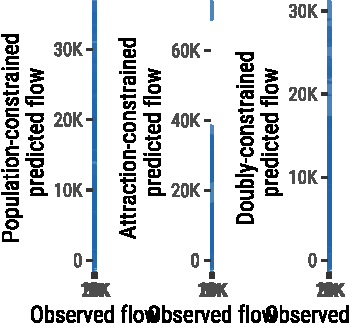
\includegraphics{region-quarto-template_files/figure-pdf/unnamed-chunk-9-1.pdf}

\hypertarget{statistical-gravity-models}{%
\subsection{Statistical gravity
models}\label{statistical-gravity-models}}

Statistical models offer a flexible and robust framework to estimate
Equation~\ref{eq-1} and a battery of summary indicators to assess
calibrated models. We can assess both their inferential and predictive
capabilities. We will start by using a linear regression model (LRM) to
build the foundations before progressing to more sophisticated modelling
approaches. This approach does not preserve the multiplicative nature of
Equation~\ref{eq-1}. Rather, it assumes linearity in the relationship
between the flows and the parameters of mass and distance, but it
provides an intuitive framework that we can use to understand more
complex modelling frameworks.

\hypertarget{linear-regression-model}{%
\subsubsection{Linear regression model}\label{linear-regression-model}}

We estimate a LRM assuming that the commuting flows as a linear function
of the population size at both origins and destinations as a proxy for
the mass parameters of Equation~\ref{eq-1}, and distance between LDA
centroids. We first focus on understanding the default R summary output.
The first block indicates the equation fitted via LRM. The second block
reports the residuals, revealing that the largest difference between
observed flows and the model's predicted flows is over 22 thousand. The
third block shows the coefficient estimates representing the
relationship between the flows and each predictors and their associated
standard errors, t values and p-values. The fourth block displays
overall model diagnostics indicating how well the model can predict the
observed flows. The higher the \(R^{2}\) statistics, the better the
model fit indicating that the model does a good job at fitting the data.
A p-value for the \(F\) statistic smaller than 0.05 is often considered
to be strong evidence to reject the null hypothesis that all of the
relationships of the set of predictors included in the model are
simultaneously zero.

\begin{Shaded}
\begin{Highlighting}[]
\NormalTok{lrm }\OtherTok{\textless{}{-}} \FunctionTok{lm}\NormalTok{(count }\SpecialCharTok{\textasciitilde{}}\NormalTok{ population\_o }\SpecialCharTok{+}\NormalTok{ population\_d }\SpecialCharTok{+}\NormalTok{ distance\_km,}
          \AttributeTok{data =}\NormalTok{ df)}
\FunctionTok{summary}\NormalTok{(lrm)}
\end{Highlighting}
\end{Shaded}

\begin{verbatim}

Call:
lm(formula = count ~ population_o + population_d + distance_km, 
    data = df)

Residuals:
    Min      1Q  Median      3Q     Max 
 -384.0  -105.2   -77.1   -55.9 22872.3 

Coefficients:
               Estimate Std. Error t value            Pr(>|t|)    
(Intercept)  1.93264119 7.37825298   0.262               0.793    
population_o 0.00021665 0.00001720  12.592 <0.0000000000000002 ***
population_d 0.00023818 0.00001713  13.907 <0.0000000000000002 ***
distance_km  0.00047255 0.00049737   0.950               0.342    
---
Signif. codes:  0 '***' 0.001 '**' 0.01 '*' 0.05 '.' 0.1 ' ' 1

Residual standard error: 607.5 on 69648 degrees of freedom
Multiple R-squared:  0.004866,  Adjusted R-squared:  0.004823 
F-statistic: 113.5 on 3 and 69648 DF,  p-value: < 0.00000000000000022
\end{verbatim}

Interpretation: the overall model diagnostics indicate that the model
does not do a good job fitting the observed flows. A \(R^{2}\) of
\(0.0048\) indicates that model only explains \(0.48\)\% of the
variability in commuting flows. A \(F-statistics\) of 113.5 with a
\(p-value\) of less than 0.05 indicates that all coefficients for the
predictor are statistically different from zero at lower than the 5\%
level of significance. In terms of the individual coefficients, only the
coefficients for population size are statistically significant and
positive. As predicted by the gravity model, the positive sign indicates
that the size of commuting flows increase with the size of populations
at origins and destinations. The coefficient for population at origin
suggests that the expected size of commuting flow increases by
\(0.00021\) for every additional person in the population at the origin.
Surprisingly, albeit statistically insignificant, the coefficient for
distance is positive. This contrasts with the key assumption of the
gravity model that distance exerts a negative effect on spatial
interactions. This does not seem to be the case for commuting flows in
the UK where people travel to work from very far distances, particularly
to London. The coefficient for the intercept indicates that the average
expected commuting count is 1.93 people.

\hypertarget{log-linear-regression-model}{%
\subsubsection{Log-linear regression
model}\label{log-linear-regression-model}}

\[
log(T_{ij}) = log(\kappa) + \mu log( M_{i} )+ \gamma log( M_{j} ) - \beta log( D_{ij} )
\]

\begin{verbatim}

Call:
lm(formula = log(count) ~ log(population_o) + log(population_d) + 
    log(distance_km), data = df)

Residuals:
    Min      1Q  Median      3Q     Max 
-2.5912 -1.2159 -0.4253  0.5771  7.8842 

Coefficients:
                   Estimate Std. Error t value            Pr(>|t|)    
(Intercept)       -7.187371   0.217141 -33.100 <0.0000000000000002 ***
log(population_o)  0.421124   0.011617  36.250 <0.0000000000000002 ***
log(population_d)  0.315283   0.011083  28.448 <0.0000000000000002 ***
log(distance_km)   0.005887   0.010177   0.578               0.563    
---
Signif. codes:  0 '***' 0.001 '**' 0.01 '*' 0.05 '.' 0.1 ' ' 1

Residual standard error: 1.732 on 69648 degrees of freedom
Multiple R-squared:  0.02867,   Adjusted R-squared:  0.02863 
F-statistic: 685.2 on 3 and 69648 DF,  p-value: < 0.00000000000000022
\end{verbatim}

\hypertarget{logistic-regression-model-with-aggregated-data}{%
\subsubsection{Logistic regression model with aggregated
data}\label{logistic-regression-model-with-aggregated-data}}

\hypertarget{poisson-regression-model}{%
\subsubsection{Poisson regression
model}\label{poisson-regression-model}}

\begin{verbatim}

Call:
glm(formula = count ~ population_o + population_d + distance_km, 
    family = poisson, data = df)

Coefficients:
                   Estimate     Std. Error z value            Pr(>|z|)    
(Intercept)  3.813004908649 0.001154291792 3303.33 <0.0000000000000002 ***
population_o 0.000001603633 0.000000002055  780.54 <0.0000000000000002 ***
population_d 0.000001710204 0.000000001986  861.12 <0.0000000000000002 ***
distance_km  0.000004436144 0.000000082848   53.55 <0.0000000000000002 ***
---
Signif. codes:  0 '***' 0.001 '**' 0.01 '*' 0.05 '.' 0.1 ' ' 1

(Dispersion parameter for poisson family taken to be 1)

    Null deviance: 38519457  on 69651  degrees of freedom
Residual deviance: 37499031  on 69648  degrees of freedom
AIC: 37751790

Number of Fisher Scoring iterations: 8
\end{verbatim}

\emph{Constrained models}

\includegraphics{region-quarto-template_files/figure-pdf/unnamed-chunk-15-1.pdf}

\begin{verbatim}
# A tibble: 6 x 4
  count lrm_predicted_flow loglrm_predicted_flow poissonrm_predicted_flow
  <dbl>              <dbl>                 <dbl>                    <dbl>
1  1500               61.6                  1.43                     70.6
2   671               56.6                  1.41                     67.7
3  4240               70.6                  1.52                     74.8
4   398               55.3                  1.34                     67.9
5     2               75.4                  1.54                     77.6
6     4               62.4                  1.45                     70.8
\end{verbatim}

\begin{Shaded}
\begin{Highlighting}[]

\end{Highlighting}
\end{Shaded}

\hypertarget{extensions}{%
\subsection{Extensions}\label{extensions}}

\hypertarget{including-push-pull-factors}{%
\subsubsection{Including push-pull
factors}\label{including-push-pull-factors}}

\hypertarget{negative-binomial-regression-model}{%
\subsubsection{Negative binomial regression
model}\label{negative-binomial-regression-model}}

\hypertarget{generalised-linear-mixed-gravity-models}{%
\subsubsection{Generalised linear mixed gravity
models}\label{generalised-linear-mixed-gravity-models}}

\hypertarget{machine-learning-gravity-models}{%
\subsubsection{Machine learning gravity
models}\label{machine-learning-gravity-models}}


\renewcommand\refname{References}
  \bibliography{bibliography.bib}



% This is the COPYRIGHT statement for the article.
\vspace*{\fill}
\tabcolsep0mm
\noindent
\begin{tabular*}{\textwidth}{ll}
	\toprule
	\multirow{2}{19mm}{
\includegraphics[width=18mm,height=10mm]{_extensions/region-ersa/REGION/CC-BY-88x31}} & {\small \multirow{2}{328pt}{\textcopyright\  by the authors. Licensee: REGION -- The Journal of ERSA, European Regional Science Association, Louvain-la-Neuve, Belgium. This article is distri-}} \\
	& \\[-1pt]
	\multicolumn{2}{l}{\small \multirow{2}{\textwidth}{buted under the terms and conditions of the Creative Commons Attri\-bution (CC BY) license (\href{http://creativecommons.org/licenses/by/4.0/}{http://creativecommons.org/licenses/by/4.0/}).}}\\
	& \\
	\bottomrule
\end{tabular*}
\end{document}
